%! Author = leocr
%! Date = 04/01/2025

% Preamble
\documentclass[12pt]{article}

% Packages
\usepackage[top=1in, bottom=1.2in, left=1in, right=1in]{geometry}
\usepackage{amsmath}
\usepackage{upgreek}
\usepackage{graphicx}
\usepackage{subcaption}
\setlength{\parindent}{0pt}



% Document
\begin{document}
    \section{Introduction}
    The aim of this work is to estimate the parameters of the SIR model.
    In particular, I will focus on the first wave of contagion of the Coronavirus pandemic in Italy.

    \begin{figure}[h!]
        \label{fig:covid_italy}
        \centering
        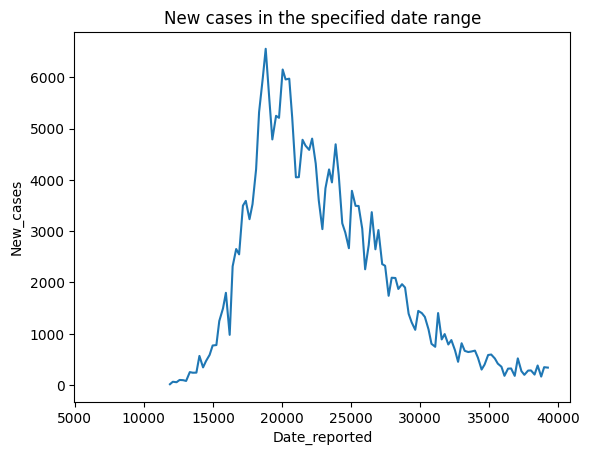
\includegraphics[width=.8\linewidth]{plots/real_data}
        \caption{New infections per day in Italy}
    \end{figure}

    \section{Model}

    \subsection{Standard SIR model}
    My first try was with the following differential equation for the total infected population:

    $$\frac{dN}{dt} = r N \left(1-\frac{N}{K}\right), \quad N(0)=N_0$$

    Which admits the following solution:

    $$N(t) = \frac{K}{1+ \left(\frac{K-N_0}{N_0}\right) e^{-rt}}$$

    That has a flex (i.e. the max of the new infections curve) in:
    $$ t^* = \frac{1}{r}\ln \left(\frac{K-N_0}{N_0}\right)$$

    To use a linear regression, the differential equation can be discretized into:
    $$ N_{t+1} = \alpha_1 N_t + \alpha_2 N_{t}^2$$

    So the parameter can be found using:
    $$ r = \alpha_1-1, \quad K= \frac{1-\alpha_1}{\alpha_2}$$

    \subsection{Bernoulli equation model}

    Recently, I found that:
    \begin{equation}
        N_{t+1} = \alpha_1 N_t + \alpha_2 N_{t}^{1 + \varepsilon}
        \label{eq:equation0}
    \end{equation}

    With $\varepsilon \in (0,1)$ would work much better to reproduce the right-hand skewness of the contagion curve.

    This equation too has a close form solution, being a Bernoulli differential equation:
    $$V = N^{-\varepsilon}, \qquad \frac{\dot V}{V} = -r \varepsilon \frac{\dot N}{N}, \quad \Rightarrow \quad \dot V = -r\varepsilon V + \frac{r\varepsilon}{K}. $$
    Which has close form solution:
    $$ V(t) = K^{-1} + \left(V_0-K^{-1}\right)e^{-r\varepsilon t} \quad \Rightarrow \quad N(t)=\frac{1}{\left(K^{-1} + \left(N_0^{-\varepsilon}-K^{-1}\right)e^{-r\varepsilon t}\right)^\varepsilon}\,.$$

    The maximum of its derivative is determined by solving:
    $$ \ddot N = -\frac{V^{-\frac{1+\varepsilon}{\varepsilon}}}{\varepsilon} \left(\ddot V -\frac{1+\varepsilon}{\varepsilon} \frac{\dot V ^2}{V}\right) \quad \to \quad t^* = \frac{1}{\varepsilon r}\ln \left(\varepsilon K N_0^{-\varepsilon}-\varepsilon\right) $$

    Where:
    $$ \dot V = -r\varepsilon\left(V_0-K^{-1}\right)e^{-r\varepsilon t}, \qquad \ddot V = (r\varepsilon)^2 \left(V_0-K^{-1}\right)e^{-r\varepsilon t}. $$

    In terms of finite differences:
    $$ V_{t+1} = \beta_0 + \beta_1 V_t,$$
    where:
    $$\beta_0 = -\alpha_2\varepsilon = \frac{r \varepsilon}{K}, \quad \beta_1=\varepsilon(1-\alpha_1) = - r\varepsilon.$$

    \subsection{Taylor expansion for small $\varepsilon$}
    Assuming $\varepsilon \simeq 0$, we can expand $N_{t}^{\,1+\varepsilon}$ as:
    \begin{equation}
        N_{t}^{\,1+\varepsilon} \simeq N_{t} \left( 1 + \varepsilon \ln N_{t} + \frac{\varepsilon^2 (\ln N_{t})^2}{2} + \frac{\varepsilon^3 (\ln N_{t})^3}{6} \right).
    \end{equation}

    So:
        \begin{equation}
        N_{t+1} = (\alpha_1 + \alpha_2) N_{t} + \varepsilon \alpha_2 N_{t}\ln N_{t} + \varepsilon^2 \alpha_2 N_{t} \frac{ (\ln N_{t})^2}{2} + \varepsilon^3 \alpha_2 N_{t} \frac{(\ln N_{t})^3}{6}.
        \end{equation}
    \newpage

    which can be useful for Ramsey testing

    \section{Estimation}\label{sec:estimation}
        \subsection{Preliminary Regression}
    Let's regress the following model with OLS:
    \begin{equation}
        V_{t+1} = \beta_0 + \beta_1 V_t
    \end{equation}
    where $V_t=N_t^{-\varepsilon}$, for different values of $\varepsilon$.

    \begin{figure}[h!]
        \centering
        \begin{subfigure}[b]{0.3\textwidth}
            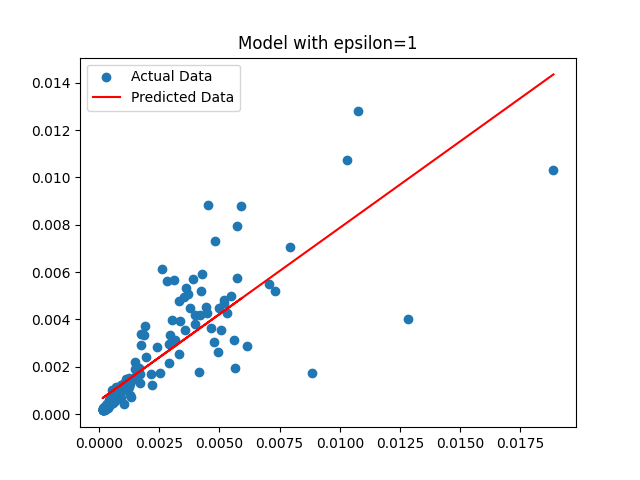
\includegraphics[width=.8\linewidth]{plots/epsilon_1}
            \caption{$\varepsilon = 1$}
        \end{subfigure} \quad
        \begin{subfigure}[b]{0.3\textwidth}
            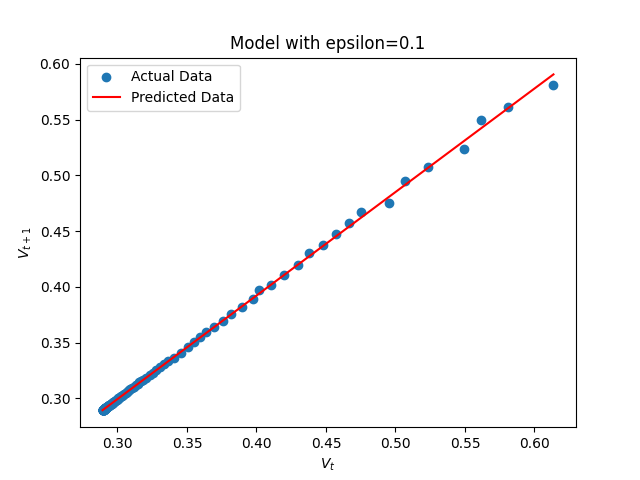
\includegraphics[width=.8\linewidth]{plots/epsilon_0.1}
            \caption{$\varepsilon = 0.1$}
        \end{subfigure} \quad
        \begin{subfigure}[b]{0.3\textwidth}
            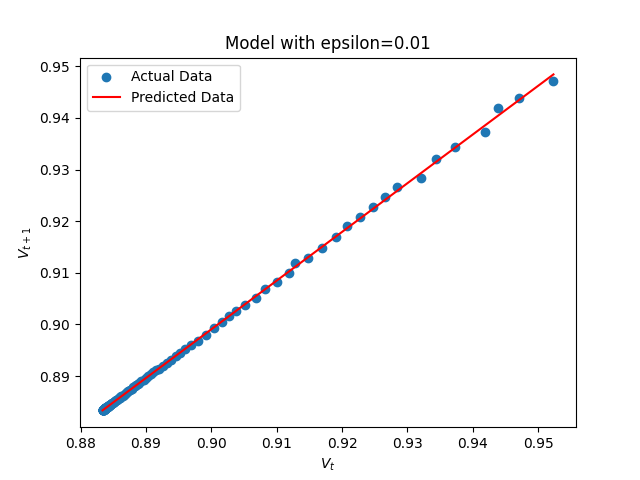
\includegraphics[width=.8\linewidth]{plots/epsilon_0.01}
            \caption{$\varepsilon = 0.01$}
        \end{subfigure}\\
        \begin{subfigure}[b]{0.3\textwidth}
            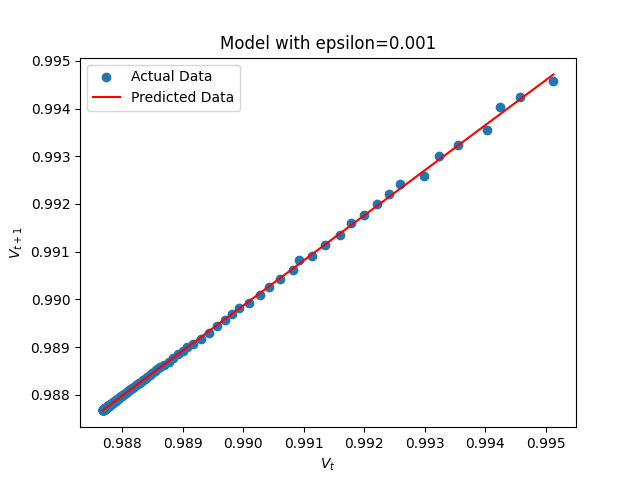
\includegraphics[width=.8\linewidth]{plots/epsilon_0.001}
            \caption{$\varepsilon = 0.001$}
        \end{subfigure} \quad
        \begin{subfigure}[b]{0.3\textwidth}
            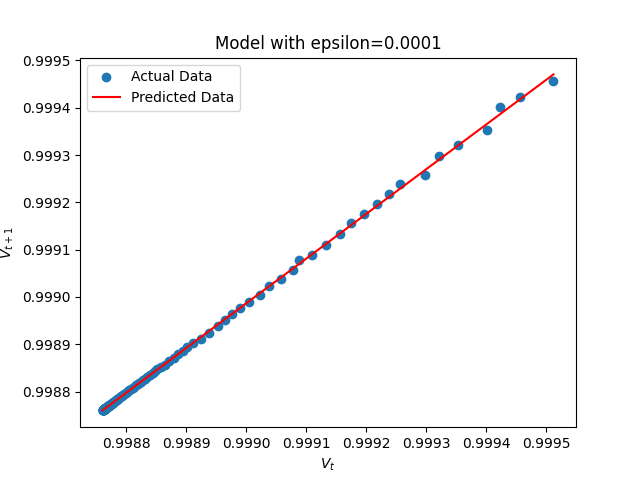
\includegraphics[width=.8\linewidth]{plots/epsilon_0.0001}
            \caption{$\varepsilon = 0.0001$}
        \end{subfigure}
        \caption{Regression Plot}
    \end{figure}

    \begin{table}[h!]
\label{tab:preliminary-regression}
\centering
    \begin{tabular}{llllll}
    \hline
                   & \varepsilon =: 1.0 & \varepsilon =: 0.1 & \varepsilon =: 0.01 & \varepsilon =: 0.001 & \varepsilon =: 0.0001  \\
    \hline
    $\beta_0$      & 0.0000*            & 0.0211***          & 0.0501***           & 0.0547***            & 0.0552***              \\
                   & (0.0000)           & (0.0006)           & (0.0013)            & (0.0014)             & (0.0014)               \\
    $\beta_1$      & 0.6348***          & 0.9278***          & 0.9433***           & 0.9446***            & 0.9447***              \\
                   & (0.0071)           & (0.0019)           & (0.0014)            & (0.0014)             & (0.0014)               \\
    \hline
    R-squared      & 0.9827             & 0.9994             & 0.9997              & 0.9997               & 0.9997                 \\
    R-squared Adj. & 0.9826             & 0.9994             & 0.9997              & 0.9997               & 0.9997                 \\
    N              & 142                & 142                & 142                 & 142                  & 142                    \\
    \hline
    \end{tabular}
    \caption{Standard errors in parentheses. \newline
$* p<0.1$, $** p<0.05$, $***p<0.01$}
\end{table}
\bigskip



    \subsection{GMM estimation with Stata}

    Let's consider the model:
    \begin{equation}
        N_{t} = \alpha_1 N_{t-1} + \alpha_2 N_{t-1}^{1 + \varepsilon} + U_t\label{eq:equation1}
    \end{equation}

    We assume that $U_t$ is mean independent of all the $N_s$ for $s\leq t-1$. For 3 parameters, at least 3 instruments are needed:

    \begin{table}[htbp]\centering
\newcommand{\sym}[1]{\ifmmode^{#1}\else\(^{#1}\)\fi}
\caption{GMM Regression Table}
\begin{tabular}{l*{4}{c}}
\hline\hline
Instruments           &\multicolumn{1}{c}{$N_1$ $N_2$}&\multicolumn{1}{c}{$N_1$ $N_2$ $N_3$}&\multicolumn{1}{c}{$N_1$ $N_2$ $N_3$ $N_4$}&\multicolumn{1}{c}{$N_1$ $N_2$ $N_3$ $N_1\ln N_1$}\\
\hline
$\alpha_1$           &       4.280         &       7.049         &       7.457         &       7.503         \\
                    &     (6.681)         &         (.)         &         (.)         &         (.)         \\
\hline
$\alpha_2$           &      -2.528         &      -4.981\sym{***}&      -5.466\sym{***}&      -5.474\sym{***}\\
                    &     (6.514)         &    (0.0550)         &    (0.0453)         &    (0.0493)         \\
\hline
$\varepsilon$       &      0.0210         &      0.0157\sym{***}&      0.0135\sym{***}&      0.0140\sym{***}\\
                    &    (0.0436)         &  (0.000896)         &  (0.000672)         &  (0.000730)         \\
\hline
J                   &                     & 252496718.1         & 161236752.4         & 209017433.8         \\
J\_df                &           0         &           2         &           3         &           3         \\
rank                &           3         &           2         &           2         &           2         \\
\hline\hline
\multicolumn{5}{l}{\footnotesize Standard errors in parentheses}\\
\multicolumn{5}{l}{\footnotesize \sym{*} \(p<0.05\), \sym{**} \(p<0.01\), \sym{***} \(p<0.001\)}\\
\end{tabular}\label{tab:gmm_table}
\end{table}


    All the model failed to converge in Stata (tried with different criteria, but without luck).

    \begin{figure}
        \centering
        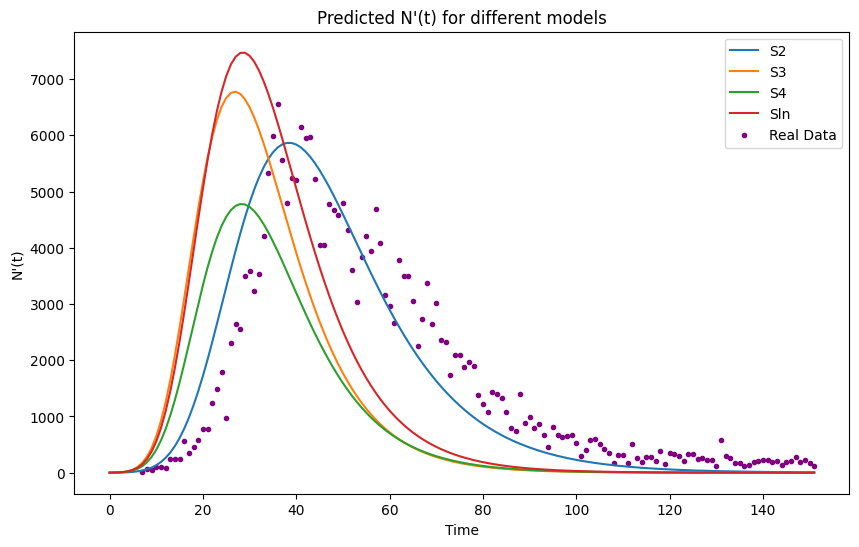
\includegraphics{plots/gmm_stata}
    \end{figure}

    \subsection{GMM estimation with grid search}

    I therefore implemented the (iterative) GMM in python, with the minimization done by grid search on the parameters:


    \subsection{Ramsay Test}




% \dot V(t) = -r\varepsilon\, \left(V_0-K^{-1}\right)e^{-r\varepsilon t}

For P-0 consider the stationary distribution as $t \to \infty $ and estimate t* as an average with that distribution



\end{document}